% --------------------------------------------------------------------------
% Template for DCASE 2017 paper; to be used with:
%          dcase2017.sty  - DCASE 2017 LaTeX style file, and
%          IEEEbib.bst - IEEE bibliography style file.
% Adapted from spconf.sty and waspaa15.sty
% --------------------------------------------------------------------------

\documentclass{article}
\usepackage{dcase2017,amsmath,graphicx,url,times,booktabs, tabularx}

% Example definitions.
% --------------------
\def\defeqn{\stackrel{\triangle}{=}}
\newcommand{\symvec}[1]{{\mbox{\boldmath $#1$}}}
\newcommand{\symmat}[1]{{\mbox{\boldmath $#1$}}}

% Title.
% --------------------
\title{A HIERARCHIC MULTI-SCALED APPROACH FOR RARE SOUND EVENT DETECTION}

% Single addresses (uncomment and modify for single-address case).
% --------------------
% \name{Author(s) Name(s)\thanks{Thanks to XYZ agency for funding.}}
% \address{Author Affiliation(s)}
%
% For example:
% ------------
% \address{School\\
%       Department\\
%       Address}

% Two addresses
% --------------------
%\twoauthors
%  {John Doe\sthanks{Thanks to ABC agency for funding.}}
%    {Fictional University\\
%Computer Science Dept., 2133 Long Road\\
%     Gotham, NY 10027, USA \\
%     john@fictional.edu}
%  {Maria Ortega\sthanks{Thanks to XYZ agency for funding.}}
%    {  University of the Imagination \\
%     Big Engineering Building, 8765 Dream Blvd. \\
%     New Chicago, IL 60626, USA \\
%     maria@imagination.edu}

% Authors in two lines, use in case of many authors with many affiliations (uncomment and modify).
% --------------------
 \name{Fabio Vesperini$^{1}$,
       Diego Droghini$^{1}$,
       Daniele Ferretti$^{1}$
       }
 \secondlinename{	
 	   Emanuele Principi$^{1}$,  
       Leonardo Gabrielli$^{1}$,
       Stefano Squartini$^{1}$, 
       Francesco Piazza$^{1}$
       }
       % fixed *.sty to allow names on multiple lines
 \address{$^1$ Politecnic University of Marche, Information Engineering  Dept., Ancona, Italy,\\ \{d.droghini, v.vesperini, d.ferretti\}@pm.univpm.it\\   
 		\{e.principi, l.gabrielli, s.squartini, f.piazza\}@univpm.it\\       
}
  

\begin{document}

\ninept
\maketitle

\begin{sloppy}

\begin{abstract}
We propose a system for rare sound event detection using hierarchical and multi-scaled approach based on Multi Layer Perceptron (MLP) and Convolutional Neural Networks(CNN). 
It is our contribution to the rare sound event detection task of the IEEE AASP Challenge on  Detection and Classification of Acoustic Scenes and Events (DCASE2017). The task consists on detection of event onset from artificially generated mixtures. Acoustic features are extracted from the acoustic signals, successively first event detection stage is performed by an MLP architecture which proposes contiguous blocks of frames to the second stage. The CNN refines the event detection of the prior network, intrinsically operating on a multi-scaled resolution and discarding blocks that contain background wrongly classified by the MLP as event. Finally the effective onset time of the active event is obtained.
The achieved overall error rate and F-measure on the development testset are respectively equal to 0.18 and 90.9\%.
\end{abstract}

\begin{keywords}
DCASE2017, Rare sound event detection, MLP, CNN, \textit{LogMel}
\end{keywords}


\section{Introduction}
\label{sec:intro}

\label{sec:format}
%2 aprole su soude evet det
%2 parole su nostri lavori novelty + (fall detection)
%2 parole su dcase daaset + ref a loro


The field of computational auditory scene analysis (CASA) cover many topics. Nowadays, one of the most importat topic is the automatic sound event detection (SED). SED is defined as the task of analysing a continuous audio
signal in order to extract a description of the sound events
occurring in the audio stream. This description is commonly
expressed as a label that marks the start, the ending, and the
nature of the occurred sound (e.g., children crying, cutlery,
glass jingling).
Task 2 of DCASE challange 2017 \cite{dcase2017web} consists in determining the precise onset of three types of sounds: babycry, glassbreak and gunshoot. 

\section{Proposed Method}
\label{sec:pagelimit}
%algo composto da 4 stadi principali: eat extr - event detection - multiscaled detection refinement - event onset annotation 
The proposed system is a hierarchical algorithm composed of four main stages: the acoustic features extraction, the first event detection stage performed by a Multi Layer Perceptron Neural Network (MLP) and a dedicated smoothing procedure of its output and a refinement of the previous decision stage performed by a Convolutional Neural Network (CNN) which intrinsically operates on a multi-scaled resolution and discards blocks that contain background wrongly classified by the MLP as event. Finally by means of a statistical decision procedure the effective onset frame of the active event is obtained.

\subsection{Feature Extraction}
The feature extraction stage operates on mono audio signals sampled at 44.1 kHz. For our purpose, we exploit \textit{LogMel} as feature set, following results obtained for the baseline system of the DCASE2017 challenge \cite{DCASE2017challenge}. \textit{LogMel} coefficients are obtained by filtering the magnitude spectrum with a filter-bank composed of 40 filters evenly spaced in the mel frequency scale and then computing the logarithm of the energy of each band. The used frame size is equal to 40 ms and the frame step is equal to 20 ms. 
The range of feature values is then normalized according to the mean and the standard deviation computed on the training sets of the neural networks.
\subsection{Multilayer Perceptron Neural Network}
The MLP artificial neural network was introduced in 1986 \cite{Rumelhart86-LRB}. The main element is the artificial neuron, consisting in an activation function applied to the sum of the weighted inputs. Neurons are then arranged in layers, with feed forward connections from one layer to the next. The supervised learning of the network makes use of the stochastic gradient descent with error back-propagation algorithm. The output layer is formed by two units with the \textit{softmax} non-linear function, defined as:  $\varphi(x_k) = e^{x_k}/\sum_{j=1}^{2}e^{x_j}$ for $k=1,2$. The outputs of the softmax layer represent the probabilities that a sample belongs to the background or the event class. 
The network is designed to consider a temporal context, thus the current feature vector $\mathbf{x}[t]$ at the frame index $t$ and a context size equal to $C$ is concatenated with the previous feature vectors obtaining:
\begin{equation}
\mathbf{x}[t] =  \{\mathbf{x}[t - c],\ldots,\mathbf{x}[t-1],\mathbf{x}[t]\},
\end{equation}
with $c = 1, \dots, C$.

\subsubsection{Post Processig}
As network output signal we consider the output of the neuron corresponding to the event class. It is convolved with an exponential decay window of length ($w$), then it is processed with a sliding median filter and finally a threshold $\theta$ is applied.

\subsection{Convolutional Neural Network}
lavora su base chunk 20 frame: organizzazione input (chunk da 20 non overlappati) e label 
descrizione di come lavorano i kernel per efatizzare la multiresolution approach
cleassificazione chunk ovellappati (chunk size -1 )

CNN is a feed-forward neural network \cite{Yann-cnn-1998} usually composed of three types of layers: convolutional layers, pooling layers and layers of neurons. The convolutional layer performs the mathematical operation of convolution between a multi-dimensional input and a fixed size kernel. Successively, a non-linearity is applied element-wise. The kernels are generally small compared to the input, allowing CNNs to process large inputs with few learnable parameters. Successively, a pooling layer is usually applied, in order to reduce the feature map dimensions. Finally, at the top of the network, an MLP layer is applied.
The aims of the CNN is to discriminate the event, selected from the previous network, from the background. The network is trained as a biclass classifier on non-overapped audio chunk of logmel frames with resulting 2D input dimension of 40x20. In the case of audio task, CNN usually exploits the temporal evolution of the signal \cite{thomas2014analyzing} due of is nature. 
In the classification phase the audio event are evaluated based on chunk 40x20 with an overlapp of 95\% (1 frame shift). This leads to an analisy of the audio event at different time and frequency resolution with respect to previous network. 
\subsubsection{Post Processig }
per ogni seq analizzo tutti gli eventi. Scarto quelli classificati con bck . Prendo il primo evento classificato come non bck perche lo scopo è beccare l onseth
\section{Experimental Set-Up}
\label{sec:pagestyle}
According to the DCASE 2017 guidelines, the performance of the proposed algorithm has been assessed firstly by using the development dataset for training and validation of the system. Then, a blind test on the provided evaluation dataset was performed with the model achieving the highest performance. The performance metric of the DCASE 2017 challenge is the event-based error rate calculated using onset-only condition with a collar of 500 ms. Additionally, event-based F-score with a 500 ms onset-only collar was calculated. Detailed information on metrics calculation is available in \cite{Mesaros2016_MDPI}. 

\subsection{MLP Event Detection Stage}
%random search per la ricerca di parametri di layout della rete NN: validation split del dcase 
%Per goni rete è stata effettuata un gridsearch sui parametri di post processing per l ottimizzazione del ER
%E' stata selezionata la rete che ha ottenuto l' ER più basso
%La rete selezionata è stata trainata nuovamente con aggiungendo al trainset delle sequenze  contenente gunshot per bilanciare i secondi di materiale degli eventi
The performance of the MLP event detection stage has been assessed by exploring the networks topology with a random search strategy \cite{bergstra2012random}. Table XX shows the parameters explored in the random search, as well as the prior distribution and ranges. The
number of explored parameters sets depends on the wideness of the search space. In this work, we explored 200 sets of layout parameters for the MLP event detection. For each of these a grid search was performed in order to find the post-processing parameters yelding the minimum error rate. Investigated parameters in the grid search were: exponential window $w$, median filter kernel $k$ and threshold $\theta$. The respective ranges are reported in Table XX.

%TODO: add table with random search parameters and distributions + gridsearch ranges
Because of the fast decay of "gun shot" sound, we the noticed that the audio segments containing this event were in small number with respect to the other samples. For this reason we trained the event detector MLP obtained from the random seach with an extended dataset, including 500 newly generated mixtures containing the "gun shot" sound event.
At the end of the validation stage of the system the trained once again the neural network including all the mixtures in the development dataset furnished with the DCASE 2017 challenge package and the aforementioned 500 newly generated containing the "gun shot" sound event for a total of 3487 audio sequences.

\subsection{Multiscaled Refinement Decision Stage}
Per trainare la cnn abbiamo data in ingresso alla prima rete delle sequenze audio di solo bck. Gli eventi selezionati da questa rete rappresentano il materiale di training
della classe bck per la cnn. Per le altre classi di eventi abbbiamo preso le porzioni di soli eventi mixed to bck relativi alle mixture fornite dal dcase e gli isolated events.

Abbiamo generato una stratified validation split del dataset appena descritto. 
Abbiamo effetuato una valutazione della cnn subase evento con la fmeasure.
Finally, sul validati

\subsection{Evaluation Phase}
%Descrizione con img della fase di valutazione
%Scelta th 0.20 invece che 0.25: per favorile meno deletion a discapito delle insertion. La cnn pensa a eliminare le insertion classificandole come bck
Once the best performing models were found, during the validation stage we performed a fine tuning of the post processing parameters of the event detection MLP in order to assess the performance of the whole system. In fact, the hierarchical architecture of the algorithm permits to set a lower threshold in the first decision stage in order to reduce the deletions to the detriment of some insertions that will be removed by the successive decision stage. The parameters of the best performing system are reported in Table YY.
\section{Results}
Error rate su base evento prima rete: 
Fmeasure cnn:

Risultato finale 0.18 più report per classi ( evetuale discussio sui babycry che nn vengono classificati bene )
\label{sec:typestyle}

\subsection{Real Scenario application}
Descrizione scenario reale: trainig cnn su 4 classi
risultato finale 0.23

\section{Conclusion}
\label{sec:majhead}


Fig.~\ref{fig:results}. 

% Below is an example of how to insert images. 
% -------------------------------------------------------------------------
\begin{figure}[t]
  \centering
  \centerline{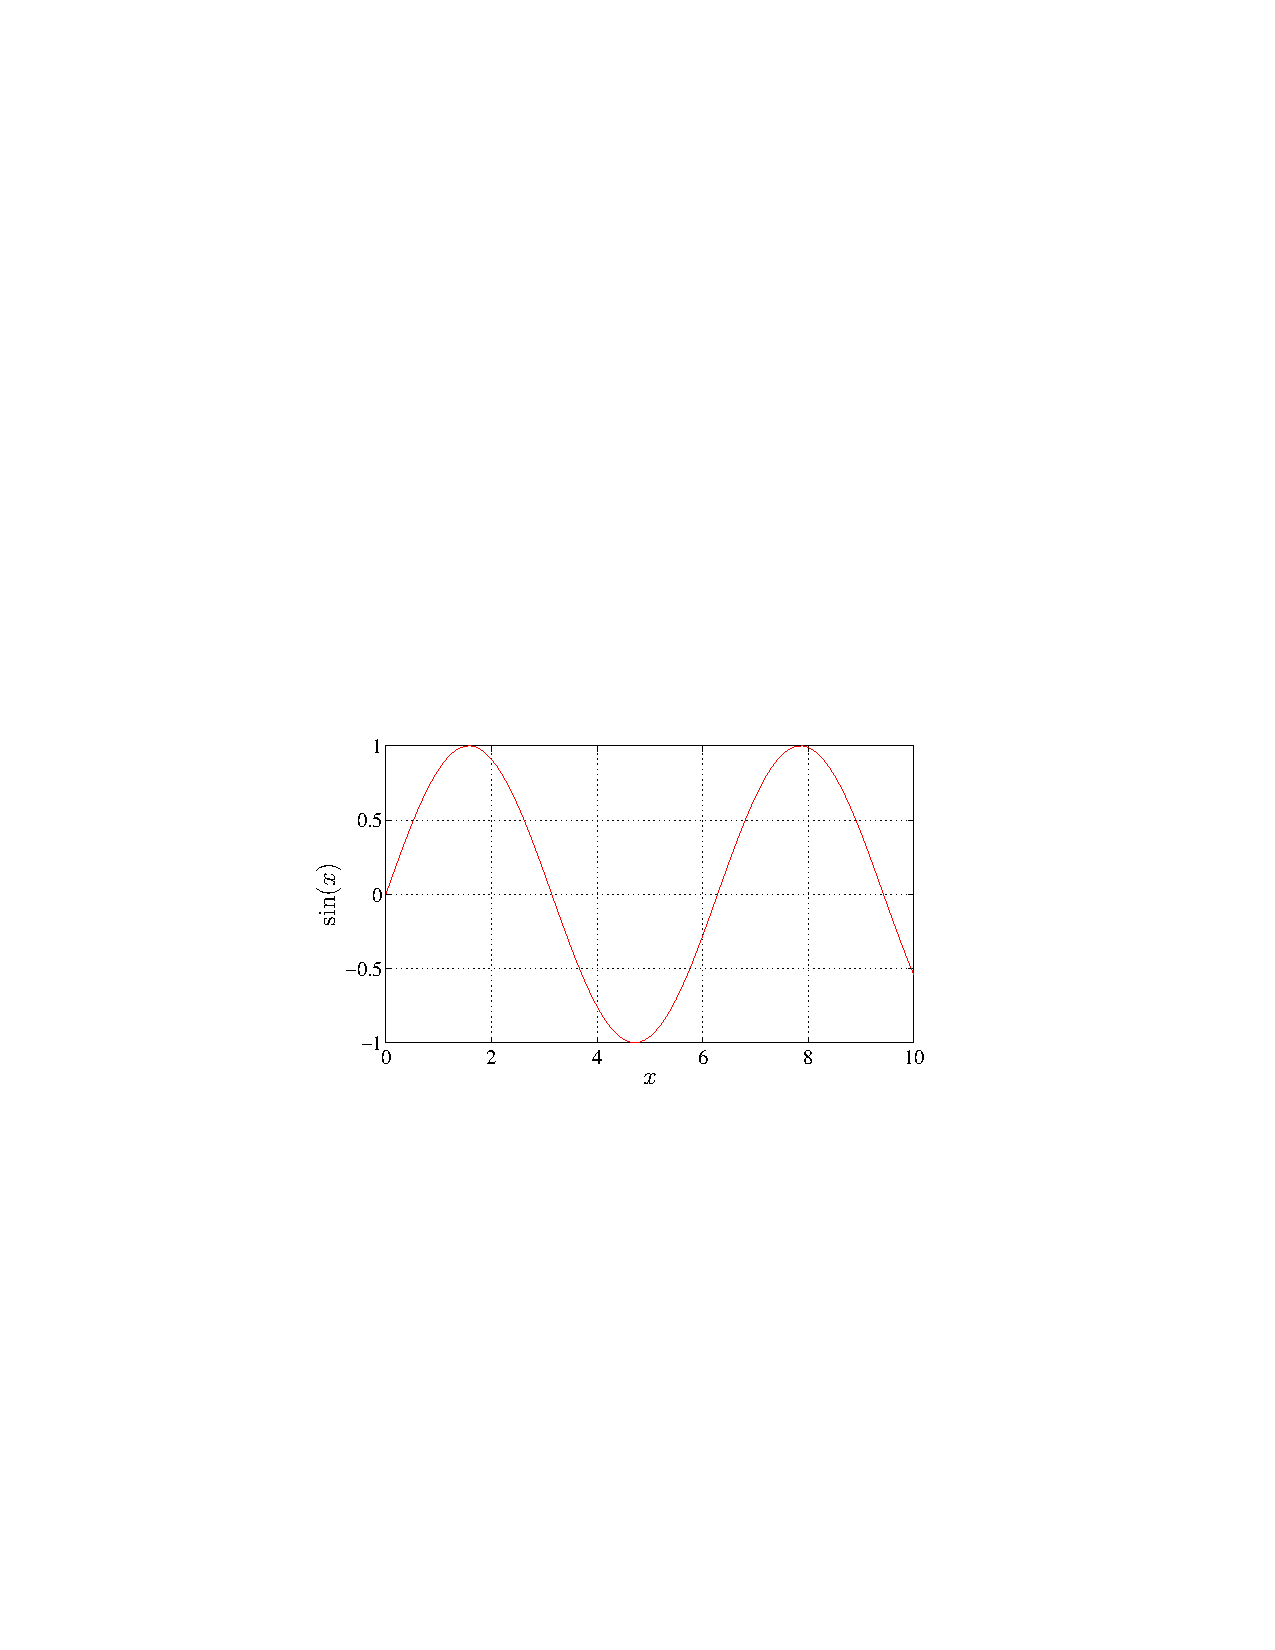
\includegraphics[width=\columnwidth]{fig1a}}
  \caption{Example of a figure with experimental results.}
  \label{fig:results}
\end{figure}

\begin{equation}
  \label{eqn:wave_equation}
    \Delta^2p(x,y,z,t)-
    \displaystyle\frac{1}{c^2}\frac{\partial^2p(x,y,z,t)}{\partial t^2}=0,
\end{equation}



% -------------------------------------------------------------------------
% Either list references using the bibliography style file IEEEtran.bst
\bibliographystyle{IEEEtran}
\bibliography{refs}
%
% or list them by yourself
% \begin{thebibliography}{9}
% 
% \bibitem{dcase2016web}
%   \url{http://www.cs.tut.fi/sgn/arg/dcase2016/}.
%
% \bibitem{IEEEPDFSpec}
%   {PDF} specification for {IEEE} {X}plore$^{\textregistered}$,
%   \url{http://www.ieee.org/portal/cms_docs/pubs/confstandards/pdfs/IEEE-PDF-SpecV401.pdf}.
%
% \bibitem{PDFOpenSourceTools}
%   Creating high resolution {PDF} files for book production with 
%   open source tools, 
%   \url{http://www.grassbook.org/neteler/highres_pdf.html}.
%
% \bibitem{eWilliams1999}
% E. Williams, \emph{Fourier Acoustics: Sound Radiation and Nearfield Acoustic
%   Holography}. London, UK: Academic Press, 1999.
% 
% \bibitem{ieeecopyright}
%   \url{http://www.ieee.org/web/publications/rights/copyrightmain.html}.
%
% \bibitem{cJones2003}
% C. Jones, A. Smith, and E. Roberts, ``A sample paper in conference
%   proceedings,'' in \emph{Proc. IEEE ICASSP}, vol. II, 2003, pp. 803--806.
% 
% \bibitem{aSmith2000}
% A. Smith, C. Jones, and E. Roberts, ``A sample paper in journals,'' 
%   \emph{IEEE Trans. Signal Process.}, vol. 62, pp. 291--294, Jan. 2000.
% 
% \end{thebibliography}


\end{sloppy}
\end{document}
\grid
